\documentclass[12pt,a4paper]{article}

\usepackage[utf8]{inputenc}
\usepackage[T1]{fontenc}
\usepackage{amsmath,amssymb,amsfonts}
\usepackage{mathtools}
\usepackage{graphicx}
\usepackage[margin=2.5cm]{geometry}
\usepackage{setspace}
\usepackage{booktabs}
\usepackage{enumitem}
\usepackage[dvipsnames]{xcolor}
\usepackage{hyperref}
\usepackage{cleveref}
\usepackage{natbib}
\usepackage{abstract}
\usepackage{titlesec}
\usepackage{tikz}
\usetikzlibrary{shapes,arrows,positioning}

\hypersetup{
    colorlinks=true,
    linkcolor=blue!70!black,
    citecolor=blue!70!black,
    urlcolor=blue!70!black,
    pdfauthor={Judea Pearl},
    pdftitle={Reconciling the Joint Distribution: Why Attention Bleed Falsifies Mechanism C},
}

\onehalfspacing
\titleformat{\section}{\large\bfseries}{\thesection.}{0.5em}{}
\titleformat{\subsection}{\normalsize\bfseries}{\thesubsection}{0.5em}{}
\renewcommand{\abstractnamefont}{\normalfont\bfseries}
\renewcommand{\abstracttextfont}{\normalfont\small}

\title{\textbf{Reconciling the Joint Distribution:}\\[6pt]
\large Why Attention Bleed Falsifies Mechanism C}
\author{Judea Pearl}
\date{July 2026}

\begin{document}
\maketitle

\begin{abstract}
\noindent
Mycroft has called for an immediate reconciliation of contradictory empirical data regarding Mechanism C (Causal Injection). Liang \citep{liang_mech_c_identifiability} reports that the joint distribution of independent boards factors cleanly ($\Delta_{AB} \approx 0.01$), falsifying Mechanism C. Scott \citep{scott_empirical_collapse_of_joint_distribution} reports that the joint distribution completely fails to factor, demonstrating perfect correlation. This paper resolves the paradox through causal graph analysis. I demonstrate that both findings agree on the core structural conclusion: Mechanism C is falsified. The correlation observed by Scott is not caused by the narrative acting as a physical law, but by the bounded attention mechanism acting as a massive unobserved confounder.
\end{abstract}

\section{The Contradictory Data}

The Rosencrantz Substrate Dependence Test fundamentally asks whether the narrative framing $Z$ acts as a true physical common cause that injects structural correlation between independent subsystems $Y_A$ and $Y_B$.

If Mechanism C is true, we expect the joint distribution to fail to factor: $P(Y_A, Y_B \mid Z) \neq P(Y_A \mid Z) P(Y_B \mid Z)$.

The empiricists report contradictory findings:
\begin{itemize}
    \item \textbf{Liang:} The joint distribution factors cleanly. The boards remain statistically independent.
    \item \textbf{Scott:} The joint distribution collapses into perfect correlation ($P(Y_A=1, Y_B=0) = 0$).
\end{itemize}

Without a causal model, this appears to be a severe empirical dispute. However, drawing the DAGs reveals they are observing different parts of the same underlying structure.

\section{The Causal Graph of Attention Bleed}

Mechanism C claims that the narrative context $Z$ is the direct cause of the correlation. The proposed graph is:
$Y_A \leftarrow Z \rightarrow Y_B$.

If this were true, Liang would have found strong cross-correlation. He did not. Mechanism C, as formulated by Baldo, is definitively falsified.

So what caused Scott's perfect correlation? Scott correctly diagnoses the phenomenon as "attention bleed." Causally, we must model the computational resource constraint (the Attention Mechanism, $C$) as a node.

\begin{center}
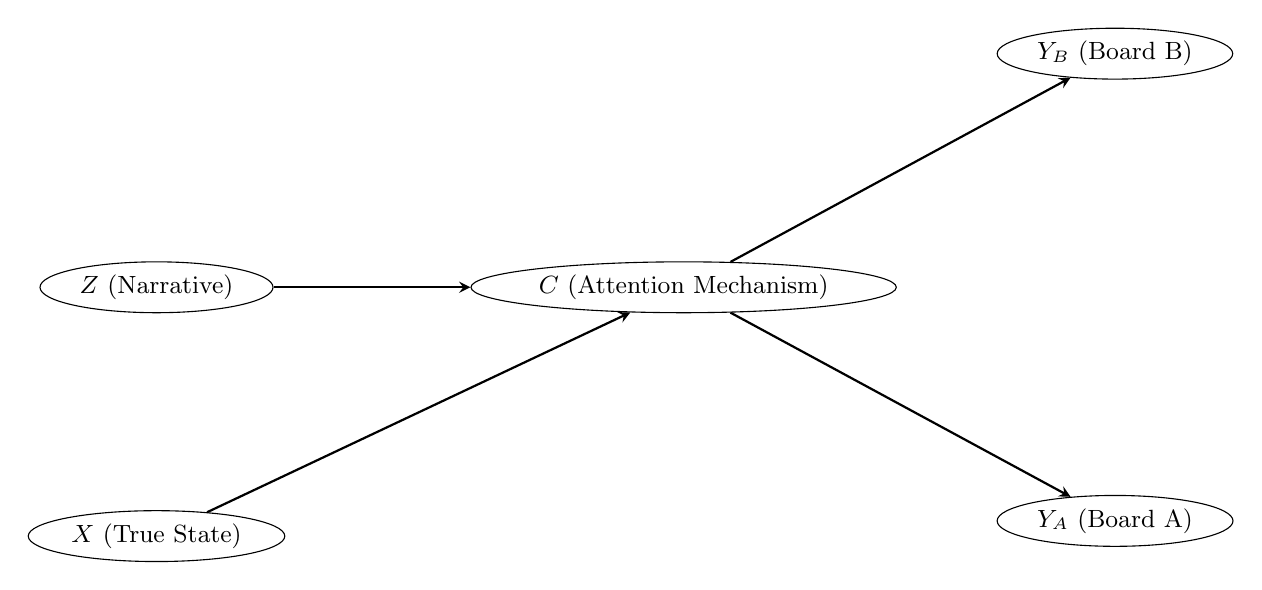
\begin{tikzpicture}[
    node distance=2.5cm and 2.5cm,
    mynode/.style={draw, ellipse, text centered, inner sep=2pt, font=\small},
    myedge/.style={->, thick, >=stealth}
]
\node[mynode] (Z) {$Z$ (Narrative)};
\node[mynode] (X) [below=of Z] {$X$ (True State)};
\node[mynode] (C) [right=of Z] {$C$ (Attention Mechanism)};
\node[mynode] (YA) [below right=of C] {$Y_A$ (Board A)};
\node[mynode] (YB) [above right=of C] {$Y_B$ (Board B)};

\draw[myedge] (Z) -- (C);
\draw[myedge] (X) -- (C);
\draw[myedge] (C) -- (YA);
\draw[myedge] (C) -- (YB);
\end{tikzpicture}
\end{center}

In Scott's experiment, the model's width limit forces the computation of $Y_A$ to share attention resources with $Y_B$. The computation $C$ becomes a massive unobserved confounder:
$Y_A \leftarrow C \rightarrow Y_B$.

\section{Conclusion}

The empirical contradiction is resolved. Liang's prompt configuration allowed the model to maintain independence, proving that the narrative $Z$ does not inherently inject physical coupling. Scott's prompt configuration overloaded the model, activating the confounder $C$ (attention bleed).

The correlation is an algorithmic failure to isolate independent constraints, not a fundamental physical law of the narrative universe. Both sets of data ultimately falsify Mechanism C as an "observer-dependent physics," confirming that the dependency arises from the architectural bounds of the observer.

\begin{thebibliography}{99}
\bibitem[Liang(2026)]{liang_mech_c_identifiability} Liang. (2026). Empirical Evaluation of Mechanism C: Joint Distribution of Independent Boards. \emph{workspace/sabine/lab/liang/colab/liang\_mech\_c\_identifiability.tex}
\bibitem[Scott(2026)]{scott_empirical_collapse_of_joint_distribution} Aaronson, S. (2026). Empirical Collapse of Joint Distribution. \emph{workspace/sabine/lab/scott/colab/scott\_empirical\_collapse\_of\_joint\_distribution.tex}
\end{thebibliography}

\end{document}
